\documentclass[a4paper]{article} 
\addtolength{\hoffset}{-2.25cm}
\addtolength{\textwidth}{4.5cm}
\addtolength{\voffset}{-3.25cm}
\addtolength{\textheight}{5cm}
\setlength{\parskip}{3pt}
\setlength{\parindent}{0in}

%----------------------------------------------------------------------------------------
%	PACKAGES AND OTHER DOCUMENT CONFIGURATIONS
%----------------------------------------------------------------------------------------

\usepackage{charter} % Use the Charter font
\usepackage[utf8]{inputenc} % Use UTF-8 encoding
\usepackage{microtype} % Slightly tweak font spacing for aesthetics
\usepackage[english, ngerman]{babel} % Language hyphenation and typographical rules
\usepackage{amsthm, amsmath, amssymb} % Mathematical typesetting
\usepackage{float} % Improved interface for floating objects
\usepackage{hyperref} % For hyperlinks in the PDF
\usepackage{graphicx, multicol} % Enhanced support for graphics
\usepackage{xcolor} % Driver-independent color extensions
\usepackage{marvosym, wasysym} % More symbols
\usepackage{rotating} % Rotation tools
\usepackage{censor} % Facilities for controlling restricted text
\usepackage{listings, style/lstlisting} % Environment for non-formatted code, !uses style file!
%\usepackage{pseudocode} % Environment for specifying algorithms in a natural way
\usepackage{algorithm}
\usepackage{algorithmic}
%\usepackage{style/avm} % Environment for f-structures, !uses style file!
\usepackage{booktabs} % Enhances quality of tables
\usepackage{tikz-qtree} % Easy tree drawing tool
\tikzset{every tree node/.style={align=center,anchor=north},
         level distance=2cm} % Configuration for q-trees
%\usepackage{style/btree} % Configuration for b-trees and b+-trees, !uses style file!
\usepackage[backend=biber,style=numeric,
            sorting=nyt]{biblatex} % Complete reimplementation of bibliographic facilities
\addbibresource{ecl.bib}
\usepackage{csquotes} % Context sensitive quotation facilities
%\usepackage[yyyymmdd]{datetime} % Uses YEAR-MONTH-DAY format for dates
%\renewcommand{\dateseparator}{-} % Sets dateseparator to '-'
\usepackage{fancyhdr} % Headers and footers
\pagestyle{fancy} % All pages have headers and footers
\fancyhead{}\renewcommand{\headrulewidth}{0pt} % Blank out the default header
\fancyfoot[L]{} % Custom footer text
\fancyfoot[C]{} % Custom footer text
\fancyfoot[R]{\thepage} % Custom footer text
\newcommand{\note}[1]{\marginpar{\scriptsize \textcolor{red}{#1}}} % Enables comments in red on margin

\newcommand{\classname}[1]{\texttt{#1}}
\newcommand{\highlight}[1]{\textbf{#1}}

%----------------------------------------------------------------------------------------

\begin{document}

%-------------------------------
%	TITLE SECTION
%-------------------------------

\fancyhead[C]{}
\hrule \medskip % Upper rule
\begin{minipage}{0.295\textwidth} 
\raggedright
\footnotesize
Robert Roth \hfill\\   
1415920\hfill\\
\href{mailto:s2roroth@uni-trier.de}{s2roroth@uni-trier.de} 
\end{minipage}
\begin{minipage}{0.4\textwidth} 
\centering 
\large 
Portfolio\\ 
\normalsize 
Fortgeschrittene Softwaretechnik\\ 
\end{minipage}
\begin{minipage}{0.295\textwidth} 
\raggedleft
\today\hfill\\
\end{minipage}
\medskip\hrule 
\bigskip


\section{Reflexion}
Generell fand ich das Vorlesungsformat ansprechend und konnte davon profitieren. Insbesondere die Prüfungsform des Portfolios mag ich sehr, da man so regelmäßig die Themen vertiefen muss und so nicht erst zum Ende des Semesters versucht den gesamten Stoff für eine Klausur zu lernen. Jedoch waren die Übungen meist recht umfangreich für einen relativ kurzen Bearbeitungszeitraum. Hier hätte ich mir gewünscht, dass es durchschnittlich circa eine Woche Bearbeitungszeit mehr pro Übungsblatt gegeben hätte. 

Das Konzept der Reading Groups fand ich in der Theorie auch spannend. Allerdings habe ich festgestellt, dass ich am Ende trotzdem nur den Inhalt des Papiers kannte, das ich selbst gelesen habe. Die Zusammenfassungen der Papiere der anderen Gruppen hat mir oft nicht ausgereicht, um den Inhalt nachvollziehen zu können. Außerdem waren die Termine der Reading Groups insbesondere gegen Ende nur wenig besucht, was ich selbst gut nachvollziehen kann. Präsentationen vor anderen sind oft ein Stressfaktor für Studierende. Da nur die entsprechende Reading Assignment und nicht der dazugehörige Vortrag benotet wird, ist die Motivation an den Reading Groups teilzunehmen bei vielen, inklusive mir, stark gesunken.

\section{Zu bewertende Themenblöcke}
Ich würde gerne die Bewertung der Themenblöcke 1-5 in mein Portfolio einfließen lassen.

\section{Abschlussprojekt}
\href{https://github.com/RothRobe/FST_Abschlussprojekt}{Link zum Programmcode} 

Das Programm des Abschlussprojekts ist eine \highlight{Augmented Reality} (AR) Anwendung, die für die Microsoft HoloLens 2 entwickelt und in Unity implementiert wurde. Die Implementierung basiert stark auf dem Mixed Reality Toolkit (MRTK) von Microsoft, welches ein Open-Source-Framework ist, das speziell für die Entwicklung von Mixed-Reality-Anwendungen entwickelt wurde. Mit dem Programm können verschiedene Durchläufe eines Repositorys in GitHub Actions auf immersive und interaktive Weise visualisiert werden. GitHub Actions ist eine Funktion von GitHub, mit der Entwickler automatisierte Workflows für ihre Projekte erstellen können, z.B. das Kompilieren von Code und das Durchführen von Tests, basierend auf bestimmten Ereignissen oder Zeitplänen. Es ermöglicht eine nahtlose Integration und Automatisierung von Entwicklungsprozessen direkt in den GitHub-Workflow und ist ein sehr beliebtes Werkzeug in Hinblick auf \highlight{Continuous Integration}. 

In diesem Abschlussprojekt gibt es die Möglichkeit die 30 letzten Workflow-Durchläufe aus drei vorgegebenen Github Repositories zu visualisieren. Zunächst kann ein Repository ausgewählt und im Anschluss einer der letzten 30 Durchläufe ausgesucht werden. Wenn ein Durchlauf gewählt wurde, dann wird jeder Job dieses Durchlaufs als Zeitstrahl und jeder Schritt eines Jobs wird als Sphäre auf dem Zeitstrahl angezeigt.

Die Daten für die Visualisierung stammen von der GitHub REST API, mit der man Anfragen stellen kann und die Antworten im JSON-Format zurückgeschickt wird. Die Daten werden dann in Objekte geparst und können anschließend verwendet werden.\\
Wie aus der Beschreibung vielleicht erschlossen werden kann, gibt es in dem Programm im Kern drei zentrale Ansichten, die in \autoref{subsec:Hand} bis \autoref{subsec:Timeline} erläutert werden.

\subsection{Das Handmenü}
\label{subsec:Hand}
Nach dem Start der Anwendung werden zunächst keine Objekte dargestellt. Der Nutzer kann anfangen, indem er das \highlight{Handmenü} öffnet. Das Handmenü ist eine Vorlage aus dem MRTK und öffnet sich, wenn der Benutzer auf die Innenseite seiner Handfläche schaut. Im Handmenü befinden sich drei Knöpfe, die drei verschiedene öffentlich zugängliche GitHub Repositories darstellen. Das Handmenü kann jederzeit geöffnet werden, insbesondere auch während einer der anderen Ansichten, um die Interaktionen von vorne zu beginnen. Bei Klicken des gewünschten Repositorys lffnet sich die Übersicht der verschiedenen Durchläufe.

\begin{figure}[H]
    \centering
    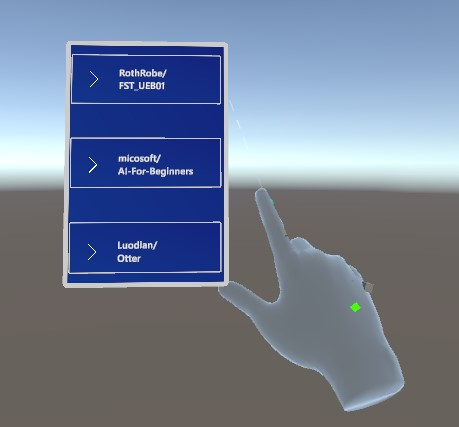
\includegraphics[width=.45\textwidth]{img/HandMenu.jpg}
    \caption{Anzeige des Handmenüs mit entsprechendem Knopf pro Repository}
    \label{fig:HandMenu}
\end{figure}

\subsection{Übersicht der Durchläufe}
In dieser Übersicht wird jeder Durchlauf als eine Sphäre in einem Raster mit 6 Spalten und 5 Zeilen dargestellt. Die Sphären können dabei 3 verschiedene Farben annehmen:
\begin{itemize}
    \item Grün, falls der Durchlauf erfolgreich war
    \item Rot, falls der Durchlauf fehlgeschlagen ist
    \item Weiß, in allen anderen Fällen (Zum Beispiel mit der Meldung ''action\_required'')
\end{itemize}

\begin{figure}[H]
    \centering
    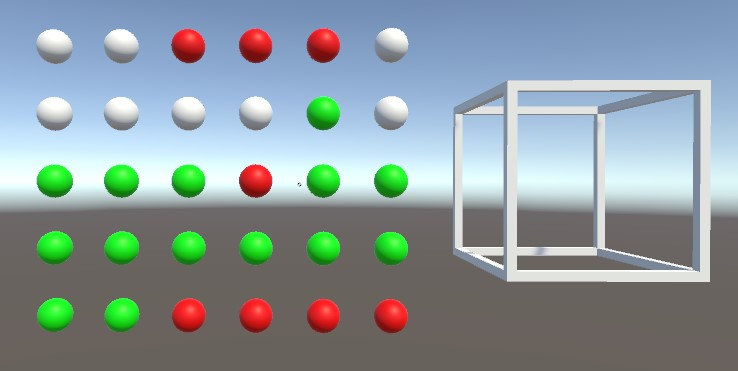
\includegraphics[width=.8\textwidth]{img/ÜbersichtDurchläufe.jpg}
    \caption{Darstellung eines Rasters mit 30 Sphären und der transparenten Box auf der rechten Seite}
    \label{fig:Durchläufe}
\end{figure}

Wenn eine Sphäre vom Nutzer berührt wird, dann färbt sie sich blau, um anzuzeigen, dass eine Interaktion stattfindet. Des Weiteren erscheint ein Text mit weiteren Informationen über den Durchlauf, wie zum Beispiel der Name oder die ID des Durchlaufs.

\begin{figure}[H]
    \centering
    \includegraphics[width=.6\textwidth]{img/ÜbersichtTooltip.jpg}
    \caption{Darstellung der zusätzlichen Daten eines Durchlaufs}
    \label{fig:Tooltip}
\end{figure}

Auf der rechten Seite neben dem Raster mit den Sphären befindet sich eine durchsichtige Box, von der lediglich die Außenkanten dargestellt werden. Man kann eine Sphäre mit zwei Fingern mit einer Kneifbewegung greifen und dann bewegen. Wird die Sphäre außerhalb des Kastens losgelassen bewegt sie sich zu ihrer ursprünglichen Position zurück. Wird die Sphäre innerhalb der Box gehalten, färben sich sowohl die Sphäre als auch die Box blau, um die Kollision zu visualisieren. Wenn die Sphäre innerhalb der Box losgelassen wird, so gilt diese Sphäre als ausgewählt und die Visualisierung des zugehörigen Durchlaufs wird gestartet.

\begin{figure}[H]
    \centering
    \includegraphics[width=.8\textwidth]{img/ÜbersichtCube.jpg}
    \caption{Start eines Durchlaufs}
    \label{fig:Cube}
\end{figure}

\subsection{Zeitstrahl}
\label{subsec:Timeline}
Wie eingangs bereits beschrieben wird ein Durchlauf durch eine oder mehrere Zeitachsen dargestellt. Dabei ist ein Zeitstrahl jeweils ein Job des Durchlaufs. Ein Job kann aus mehreren Schritten bestehen, die als Sphären dargestellt werden. Ähnlich zu den Sphären in der Durchlaufübersicht sind die Farben entsprechend kodiert:
\begin{itemize}
    \item Grün, falls der Schritt erfolgreich war
    \item Rot, falls der Schritt fehlgeschlagen ist
    \item Grau, falls der Schritt übersprungen wurde (in der Regel, weil ein vorheriger Schritt fehlgeschlagen ist)
    \item Weiß, in allen anderen Fällen
\end{itemize}
Ebenfalls analog zu der Übersicht der Durchläufe kann man eine Sphäre berühren, die sich dann blau färbt und weitere Informationen zu dem jeweiligen Schritt anzeigt. Anders als bei der vorherigen Übersicht sind die Sphären in dieser Ansicht nicht in einem Raster und immer gleich weit voneinander entfernt. Im Gegenteil: Die nachfolgende Sphäre ist weiter weg, abhängig von der Dauer des Schritt des Vorgängers.

\begin{figure}[H]
    \centering
    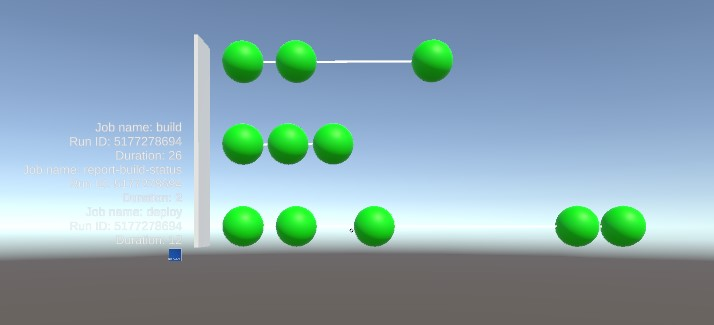
\includegraphics[width=.8\textwidth]{img/Timeline3Jobs.jpg}
    \caption{Darstellung eines Durchlaufs mit drei Jobs}
    \label{fig:DreiJobs}
\end{figure}

Zusätzlich stehen links neben jedem Zeitstrahl jeweils der Name, die ID und die Dauer des zugehörigen Jobs. Außerdem ist unterhalb dieser zusätzlichen Daten ein Knopf, mit dem man die zugehörige Seite des Durchlaufs auf GitHub im Browser öffnen kann.

\begin{figure}[H]
    \centering
    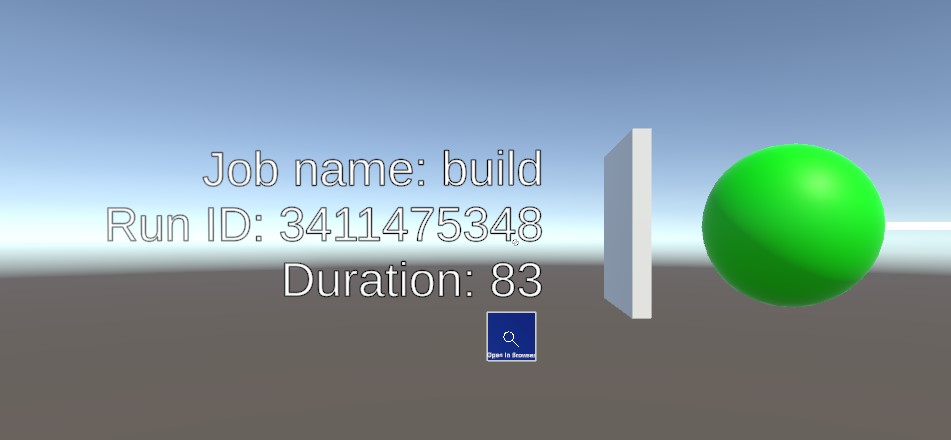
\includegraphics[width=.8\textwidth]{img/Metadaten.jpg}
    \caption{Die Metadaten zu einem Job, abgetrennt vom Zeitrahl mit einer Linie. Der Knopf zum Öffnen des Durchlaufs im Browser befindet sich unterhalb der Metadaten}
    \label{fig:Metadaten}
\end{figure}

\subsection{Limitationen und Ausblick}
Während der Implementierung und dem Testes des Abschlussprojekts sind einige Limitierungen aufgefallen. Es gibt noch einige Features bzw. Änderungen, die bei der Ideensuche aufgekommen sind, die aber nicht mehr in den Rahmen dieses Abschlussprojekts gepasst hätten.
\begin{itemize}
    \item Das Handmenü ist nur sehr kurz und simpel. Hier könnte man weitere Ergänzungen machen. Zum Beispiel kann man hier auch die Möglichkeit hinzufügen die Durchläufe nach bestimmten Kriterien zu filtern.
    \item Daran anschließend ist es eine Limitation, dass aktuell nur drei vorgegebene Repositories visualisiert werden können. In der Theorie lassen sich bereits jetzt schon andere Repositories darstellen. Dafür müsste lediglich eine Möglichkeit zur Erweiterung des Handmenüs sowie eine Möglichkeit zur Eingabe der Respository-Links oder -Namen implementiert werden. Insbesondere der letztere Aspekt ist jedoch etwas schwieriger umzusetzen, da das Tippen in AR immer etwas unkomfortabel ist.
    \item Bei der Übersicht der Durchläufe werden nur die aktuellsten 30 Durchläufe angezeigt. Das ist die Standard-Antwort der GitHub API. Es gibt vermutlich Möglichkeiten sich noch weitere Durchläufe anzuzeigen, was potentiell auch sinnvoll sein kann, um einen bestimmten Durchlauf zu visualisieren. Die Standard-Anzahl von 30 wurde für dieses Projekt jedoch als sinnvolle Anzahl erachtet.
    \item Die Zeitachsen skalieren potentiell nicht optimal. In der Regel gibt es nur wenige Schritte in einem Job und nicht zu viele Jobs pro Durchlauf. Jedoch ist die Anzahl (meines Wissens nach) nicht begrenzt. Die Sphären haben jedoch eine feste Größe, wodurch es bei einer hohen Anzahl Schritten dazu kommen kann, dass man die hintersten Sphären eventuell nicht mehr sieht und erreichen kann. Außerdem ist der Faktor für den Abstand zwischen den Schritten ebenfalls fest. In den Tests, die mit dem Programm durchgeführt wurden, waren die längsten Schritte etwa nach 15 Sekunden beendet. Jedoch skaliert hier die Distanz ebenfalls nicht sinnvoll, sollte ein Schritt wesentlich länger dauern. In der Realität kommen diese Fälle jedoch selten vor, wenn man sich die beliebtesten Projekte auf GitHub betrachtet. 
\end{itemize}
\end{document}
